\documentclass[journal,12pt,twocolumn]{IEEEtran}

\usepackage{setspace}
\usepackage{gensymb}
\singlespacing
\usepackage[cmex10]{amsmath}
\usepackage{amssymb}
\usepackage{xurl}
\usepackage{tabularx}
\usepackage{amsthm}
\usepackage{comment}
\usepackage{mathrsfs}
\usepackage{txfonts}
\usepackage{stfloats}
\usepackage{bm}
\usepackage{cite}
\usepackage{cases}
\usepackage{subfig}
\usepackage{arydshln}
\usepackage{longtable}
\usepackage{multirow}

\usepackage{enumitem}
\usepackage{mathtools}
\usepackage{steinmetz}
\usepackage{tikz}
\usepackage{circuitikz}
\usepackage{verbatim}
\usepackage{tfrupee}
\usepackage[breaklinks=true]{hyperref}
\usepackage{graphicx}
\usepackage{tkz-euclide}
\usetikzlibrary{automata, positioning}
\usetikzlibrary{calc,math}
\usepackage{listings}
    \usepackage{color}                                            %%
    \usepackage{array}                                            %%
    \usepackage{longtable}                                        %%
    \usepackage{calc}                                             %%
    \usepackage{multirow}                                         %%
    \usepackage{hhline}                                           %%
    \usepackage{ifthen}                                           %%
    \usepackage{lscape}     
\usepackage{multicol}
\usepackage{chngcntr}
\usepackage{blkarray}

\DeclareMathOperator*{\Res}{Res}

\renewcommand\thesection{\arabic{section}}
\renewcommand\thesubsection{\thesection.\arabic{subsection}}
\renewcommand\thesubsubsection{\thesubsection.\arabic{subsubsection}}

\renewcommand\thesectiondis{\arabic{section}}
\renewcommand\thesubsectiondis{\thesectiondis.\arabic{subsection}}
\renewcommand\thesubsubsectiondis{\thesubsectiondis.\arabic{subsubsection}}


\hyphenation{op-tical net-works semi-conduc-tor}
\def\inputGnumericTable{}                                 %%

\lstset{
%language=C,
frame=single, 
breaklines=true,
columns=fullflexible
}
\begin{document}


\newtheorem{theorem}{Theorem}[section]
\newtheorem{problem}{Problem}
\newtheorem{proposition}{Proposition}[section]
\newtheorem{lemma}{Lemma}[section]
\newtheorem{corollary}[theorem]{Corollary}
\newtheorem{example}{Example}[section]
\newtheorem{definition}[problem]{Definition}

\newcommand{\BEQA}{\begin{eqnarray}}
\newcommand{\EEQA}{\end{eqnarray}}
\newcommand{\define}{\stackrel{\triangle}{=}}
\bibliographystyle{IEEEtran}
\raggedbottom
\setlength{\parindent}{0pt}
\providecommand{\mbf}{\mathbf}
\providecommand{\pr}[1]{\ensuremath{\Pr\left(#1\right)}}
\providecommand{\qfunc}[1]{\ensuremath{Q\left(#1\right)}}
\providecommand{\sbrak}[1]{\ensuremath{{}\left[#1\right]}}
\providecommand{\lsbrak}[1]{\ensuremath{{}\left[#1\right.}}
\providecommand{\rsbrak}[1]{\ensuremath{{}\left.#1\right]}}
\providecommand{\brak}[1]{\ensuremath{\left(#1\right)}}
\providecommand{\lbrak}[1]{\ensuremath{\left(#1\right.}}
\providecommand{\rbrak}[1]{\ensuremath{\left.#1\right)}}
\providecommand{\cbrak}[1]{\ensuremath{\left\{#1\right\}}}
\providecommand{\lcbrak}[1]{\ensuremath{\left\{#1\right.}}
\providecommand{\rcbrak}[1]{\ensuremath{\left.#1\right\}}}
\theoremstyle{remark}
\newtheorem{rem}{Remark}
\newcommand{\sgn}{\mathop{\mathrm{sgn}}}
\providecommand{\abs}[1]{\vert#1\vert}
\providecommand{\res}[1]{\Res\displaylimits_{#1}} 
\providecommand{\norm}[1]{\lVert#1\rVert}
%\providecommand{\norm}[1]{\lVert#1\rVert}
\providecommand{\mtx}[1]{\mathbf{#1}}
\providecommand{\mean}[1]{E[ #1 ]}
\providecommand{\fourier}{\overset{\mathcal{F}}{ \rightleftharpoons}}
%\providecommand{\hilbert}{\overset{\mathcal{H}}{ \rightleftharpoons}}
\providecommand{\system}{\overset{\mathcal{H}}{ \longleftrightarrow}}
	%\newcommand{\solution}[2]{\textbf{Solution:}{#1}}
\newcommand{\solution}{\noindent \textbf{Solution: }}
\newcommand{\cosec}{\,\text{cosec}\,}
\providecommand{\dec}[2]{\ensuremath{\overset{#1}{\underset{#2}{\gtrless}}}}
\newcommand{\myvec}[1]{\ensuremath{\begin{pmatrix}#1\end{pmatrix}}}
\newcommand{\mydet}[1]{\ensuremath{\begin{vmatrix}#1\end{vmatrix}}}
\newcommand*{\permcomb}[4][0mu]{{{}^{#3}\mkern#1#2_{#4}}}
\newcommand*{\perm}[1][-3mu]{\permcomb[#1]{P}}
\newcommand*{\comb}[1][-1mu]{\permcomb[#1]{C}}
\numberwithin{equation}{subsection}
\makeatletter
\@addtoreset{figure}{problem}
\makeatother
\let\StandardTheFigure\thefigure
\let\vec\mathbf
\renewcommand{\thefigure}{\theproblem}
\def\putbox#1#2#3{\makebox[0in][l]{\makebox[#1][l]{}\raisebox{\baselineskip}[0in][0in]{\raisebox{#2}[0in][0in]{#3}}}}
     \def\rightbox#1{\makebox[0in][r]{#1}}
     \def\centbox#1{\makebox[0in]{#1}}
     \def\topbox#1{\raisebox{-\baselineskip}[0in][0in]{#1}}
     \def\midbox#1{\raisebox{-0.5\baselineskip}[0in][0in]{#1}}
\vspace{3cm}
\title{Assignment 4}
\author{Tanay Yadav - AI20BTECH11026}
\maketitle
\newpage
\bigskip
\renewcommand{\thefigure}{\theenumi}
\renewcommand{\thetable}{\theenumi}
Download the python codes from: 
%
\begin{lstlisting}
https://github.com/tanayyadav28/EE3900-Assignments/blob/main/Assignment_4/code/Assignment_4.py
\end{lstlisting}
Download the latex-tikz codes from: 
%
\begin{lstlisting}
https://github.com/tanayyadav28/EE3900-Assignments/blob/main/Assignment_4/Assignment_4.tex
\end{lstlisting}
\section{Problem}
[Linear Forms 2.23]
Find the shortest distance between the lines:
\begin{align}
    L_1 : \vec{x} &= \myvec{1\\2\\3} + \lambda_1 \myvec{1\\-3\\2}\\
    L_2 : \vec{x} &= \myvec{4\\5\\6} + \lambda_2 \myvec{2\\3\\1}
\end{align}
\section{Solution}
Given,
\begin{align}
    \vec{A_1} &= \myvec{1\\2\\3}\\
    \vec{m_1} &= \myvec{1\\-3\\2}\\
    \vec{A_2} &= \myvec{4\\5\\6}\\
    \vec{m_2} &= \myvec{2\\3\\1}
\end{align}
The lines $L_1$ and $L_2$ are intersecting if,
\begin{align}
    \myvec{1\\2\\3} + \lambda_1 \myvec{1\\-3\\2} &= \myvec{4\\5\\6} + \lambda_2 \myvec{2\\3\\1}\\
    \lambda_1 \myvec{1\\-3\\2} - \lambda_2 \myvec{2\\3\\1} &= \myvec{4\\5\\6} - \myvec{1\\2\\3}\\
    \myvec{1 & 2\\-3 & 3\\2 & 1}\myvec{\lambda_1 \\ -\lambda_2} &= \myvec{3\\3\\3}
\end{align}
Row reducing the augmented matrix,
\begin{align}
    \myvec{1 & 2 & 3\\ -3 & 3 & 3\\ 2 & 1 & 3} &\xleftrightarrow{R_2 = R_2 + 3R_1} \myvec{1 & 2 & 3\\ 0 & 9 & 12\\1 & 2 & 3}\\
    \myvec{1 & 2 & 3\\ 0 & 9 & 12\\2 & 1 & 3} &\xleftrightarrow{R_3 = R_3 - 2R_1} \myvec{1 & 2 & 3\\ 0 & 9 & 12\\0 & -3 & -3}\\
    \myvec{1 & 2 & 3\\ 0 & 9 & 12\\0 & -3 & -3} &\xleftrightarrow{R_3 = R_3 + \frac{R_2}{3}} \myvec{1 & 2 & 3\\ 0 & 9 & 12\\0 & 0 & 1}
\end{align}
The above matrix has $rank = 3$. Hence, the given lines are skew-lines.\\
The normal to both the lines is:
\begin{align}
    \vec{n} &= \vec{m}_1 \times \vec{m}_2
\end{align}
The equation of the plane is then obtained as:
\begin{align}
    \vec{n}^T\vec{x} &= \vec{n}^T\vec{A}_2
\end{align}
The distance of the above line from $\vec{A}_2$ is obtained as:
\begin{align}
    \frac{n^T(\vec{A}_2 - \vec{A}_1)}{\norm{\vec{n}}} &= \frac{(\vec{A}_2 - \vec{A}_1)^T(\vec{m}_1 \times \vec{m}_2)}{\norm{\vec{m}_1 \times \vec{m}_2}}\\
    &= \frac{\myvec{3\\3\\3}^T\myvec{-9\\3\\9}}{\sqrt{\myvec{-9\\3\\9}^T\myvec{-9\\3\\9}}}
\end{align}
\begin{align}
    &= \frac{9}{\sqrt{171}}\\
    &= \frac{3}{\sqrt{19}}
\end{align}
Hence, the shortest distance between the given lines is $\dfrac{3}{\sqrt{19}}$.
\begin{figure}[h]
    \centering
    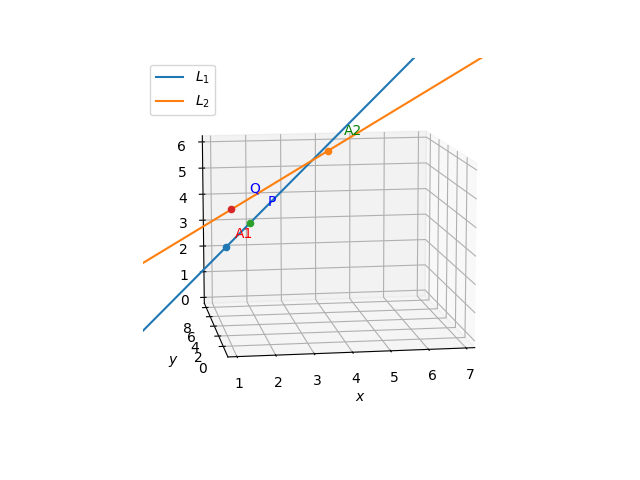
\includegraphics[scale = 0.5]{figure/Figure_1.png}
    \caption{Plot from Python Code.}
    \label{fig:my_label}
\end{figure}
\end{document}